% Stephen Marsland, July 2009
% Based on the University of Manchester class by Graham Gough

\documentclass[11pt,PhD,twoside,openright]{muthesis}

\usepackage{verbatim}
\usepackage{graphicx}
\usepackage{url}
\usepackage{hyperref}
\usepackage[round]{natbib}
\usepackage{amsmath}
\usepackage{amssymb}
\usepackage{fancyhdr}
\usepackage[small, font=sf, labelfont={sf,bf}]{caption}

\setcounter{secnumdepth}{2}
\setcounter{tocdepth}{2}
\setlength{\parindent}{0.0in}
\setlength{\parskip}{0.1in}

% Other things to set:
\subject{Computer Science}
\campus{Palmerston North} 

\begin{document}

%=====================================================================================
%  User-defined Latex Commands
%=====================================================================================

% NATBIB Bibliography Style -- better names for harvard extended styles
%\newcommand {\citen}         [1]{\citet{#1}} % as a noun eg. Blogs (2000)
%\newcommand {\citeaffixed}   [1]{\citet{#1}}
%\newcommand {\possessivecite}[1]{\citet{#1}}
%\newcommand {\urlX}[1]{\textit{#1}}          % \url doesn't like to be movable

%%----------------------------------------------------------------------------------------
% put a todo item in brackets, like   (todo: expand detail here )
\newcommand {\note}[1] {\todo[inline]{#1}}

% Put comments in a margin box
\newcommand {\thought}[1]{\marginpar{#1}}
\newcommand {\aside}[1]  {\marginpar{\tiny{#1}}}
\newcommand {\idea}[1]   {\marginpar{#1}}

% Hide some text
\newcommand {\hidden }[1]{}
\newcommand {\hide }  [1]{}

\newcommand {\product}[1]{\textit{#1}\texttrademark%
                          \index{#1@\textit{#1}}%
            }
\newcommand {\fullref}[1]{\ref{#1},~p\pageref{#1}}   % -->  4.5, p29
\newcommand {\fullrefi}[1]{\ref{#1}~(p\pageref{#1})} % inline -->  4.5 (p29)
\newcommand {\fullrefp}[1]{(sec. \fullref{#1})}      % add parentheses and sec. -> (sec. 4.5, p29)

\newcommand {\skipline} {\newline ~ \newline}
\newcommand {\gap}      {\newline ~ \newline}

\newcommand {\tab} {~~~}

\newcommand {\naive} {na\"{i}ve }
\newcommand {\degrees} {$^\circ$ }            % degree symbol

\newcommand {\LLLc} {Lifelong Learning }
\newcommand {\LLLs} {lifelong learning }
\newcommand {\LLLsn} {lifelong learning}

\newcommand {\ep} {ePortfolio}

% Registered (R) in a circle
\def\registered{{\ooalign{\hfil\raise.05ex\hbox{\tiny{R}}\hfil\crcr\mathhexbox20D}}}

% TEXT FORMATTING SHORTCUTS

\newcommand {\se}[1] {\small{\emph{#1}}}

% put a quotation in its own unindented paragraph
\newcommand {\inlinequote}[1] {\emph{#1}}

%%==========================================================================================
\newcommand {\shortquote}[1] {
   \noindent \begin{quote}
     \emph{#1}
   \end{quote}}

% Indented text, slightly smaller than usual, and italicised.
\newcommand {\smallquote}[1] {\begin{quote}\noindent\textit{#1} \end{quote}}

%%===========================================+=======================
\newcommand {\longquote}[1] {
   \noindent \begin{quotation}
     \emph{#1}
   \end{quotation}}

   
\newcommand {\bfit}[1]{\textbf{\textit{#1}}}
%% Uncomment the following lines to leave out list of figures and tables until final printing
%\figurespagefalse
%\tablespagefalse
%% Uncomment to make it singlespaced to save paper for draft printing
%\singlespace

%% Latex will put the current year on the title page by default. 
%%If you wish to change it, modify and uncomment this line
%\year=2010

\title{Lifelong Learning Supported\\ 
  By ePortfolio Process}
\author{Yuliya Bozhko}

\beforeabstract

\prefacesection{Abstract}
\begin{abstract}
\setlength{\parskip}{5pt}
Lifelong learning is seen as a self-directed pursuit of knowledge or skills that
occur throughout one's life. While this concept is not new, the importance of
\LLLs skills, in addition to academic and subject knowledge, has been
increasingly emphasised in the workplace and public policy over the last decade.
Higher education institutions, universities in particular, recognise the
importance of \LLLs and define their own strategies to promote it. Such
strategies include university development of graduate profiles which represent
the core learning outcomes, skills and qualities, that students should acquire
during their university education.

The problem identified and addressed in the current research is the lack of
comprehensive technical support solutions for \LLLs in universities. Currently,
only basic level systems are available, such as \ep~systems or accommodation of
Web 2.0 tools into university settings. However, the shortcomings of these
systems and tools, are hindering their full adoption, and as such the necessary
support for \LLLs is not available.

Through a literature review process followed by stakeholder interviews, this
thesis analyses the needs for supporting \LLLs in universities. According to
this analysis, better support is required for reflection, communication and
collaboration, development and showcasing of \LLLs skills, and tracking of
learning progress. These identified needs are then translated into requirements
that are used to create a prototype system that extends a current \ep~system,
Mahara, with new features, to provide institutional support for \LLLsn.

A number of studies, involving both lecturers and students, are conducted to
evaluate whether the prototype can be a part of the environment that provides
comprehensive support for \LLLs in universities. The results indicate that the
new features can be successfully adopted by students to help development and
understanding of \LLLs skills, address institutional graduate attributes, track
learning progress, as well as manage and share this knowledge with others. In
addition to these student-focused results, lecturers respond positively to
incorporating the prototype into their teaching. They see the opportunities for
employing the new features to provide students with the guidance through their
\LLLs journey at the university.

This research is the initial stage of providing comprehensive technical support
of \LLLs in universities. It draws attention to the influence that technology
has on teaching and learning, encourages cooperation between stakeholders, and
shows the importance of listening to the learner's voice.
\end{abstract} 

%\newpage
%\thispagestyle{empty} 
%\mbox{}

\newpage
\cleardoublepage
 
\prefacesection{Acknowledgements}
I would like to thank...

\newpage
\cleardoublepage

\prefacesection{Publications and Presentations}
\LARGE \textbf{Peer-reviewed international conferences}

\normalsize
\textbf{Bozhko, Y.}, and Heinrich, E. (2011). Concept Map-Based Framework for
Learner-Centered Knowledge Management in ePortfolios. In Proceedings of
The 11th IEEE International Conference on Advanced Learning Technologies 2011.
Athens, GA, USA.

\textbf{Bozhko, Y.}, and Heinrich, E. (2011). Enhancing ePortfolio Systems to
Better Support Lifelong Learning in Universities: Students' Perspective. In
Proceedings of World Conference on Educational Multimedia, Hypermedia and
Telecommunications 2011 (pp. 1912-1917). Chesapeake, VA: AACE.

\textbf{Bozhko, Y.}, and Heinrich, E. (2011). Academic Perspective on Enhancing
ePortfolio Systems to Better Support Lifelong Learning in Universities. In S.
Barton (Ed.), Proceedings of Global Learn Asia Pacific 2011 (pp. 137-142).
Melbourne, Australia: AACE.

\textbf{Bozhko, Y.}, and Heinrich, E. (2010). Towards a Lifelong Learning
Environment in Universities. In Z. Abas et al. (Eds.), Proceedings of Global
Learn Asia Pacific 2010 (pp. 2038-2043). Penang, Malaysia: AACE. 

\textbf{Bozhko, Y.} (2010). Towards an institutional lifelong learning
environment. DEANZ Conference 2010. Wellington, New Zealand.

\textbf{Bozhko, Y.} (2009). Lifelong learning supported by ePortfolio processes.
7th International ePortfolio Conference. London, UK.

\LARGE \textbf{Other publications}

\normalsize
Heinrich, E., and \textbf{Bozhko, Y.} (2011). The Role of Institutions in
Creating Student-Focused Virtual Learning Spaces with ePortfolio Systems. In M. Keppell,
K. Souter, and M. Riddle (Eds.), Physical and Virtual Learning Spaces in Higher
Education: Concepts for the Modern Learning Environment. IGI Global.

\textbf{Bozhko, Y.} (2011). Concept Maps for Learner-Centered Knowledge
Management in ePortfolios. 9th New Zealand Computer Science Research Student Conference
(NZCSRSC) 2011. Palmerston North, New Zealand.

\textbf{Bozhko, Y.} (2010). Towards an Institutional Lifelong Learning
Environment. 8th New Zealand Computer Science Research Student Conference (NZCSRSC) 2010.
Wellington, New Zealand.




 

\newpage
\cleardoublepage

\prefacesection{List of Abbreviations}
DSR - Design Science Research

LMS - Learning Management System

OECD - Organisation for Economic Co-operation and Development

PLE - Personal Learning Environment

UNESCO - United Nations Educational, Scientific, and Cultural Organization

VLE - Virtual Learning Environment




 

\newpage
\cleardoublepage
 
\tableofcontents
\newpage
\iftablespage
	\addvspace{10pt}
    \listoftables 
    \newpage
\fi
\iffigurespage
	\addvspace{10pt}
    \listoffigures
    \newpage
\fi

\afterpreface

\pagestyle{fancy}

\fancyhead{}
%\fancyhead[LE,RO]{\slshape \rightmark}
\fancyhead[LO,RE]{\slshape \leftmark}

\fancyfoot{} 
\fancyfoot[LE,RO]{\thepage} 
\renewcommand{\headrulewidth}{0.4pt}
\renewcommand{\footrulewidth}{0pt}

% ==============These include the actual text=======================
\chapter{Introduction\label{cha:intro}}
\epigraph{Learning is not a product of schooling, but the lifelong attempt to
acquire it.}{\textit{Albert Einstein}}
\noindent
%1215

Simply defined by the European Commission \citeyearpar{EuropeanCommission2000},
\LLLs represents all learning activities throughout lifes of individuals aimed
at improving their knowledge and skills. The concept of \LLLs has become very
popular over the last decade. The original concept has gone through a lot of
changes, through the stages of continuing, recurrent, and adult education
\citep{Jarvis2004}. On one hand, the \LLLs concept has an entirely economic
agenda, where citizens can be described as tools for economic development and
their needs are firmly tied to the needs of industry
\citep[pp.~112-114]{Carter2008}. On the other hand, as stated by UNESCO, \LLLs
is a cultural policy which influences the nature of society and promotes
positive change \citep[pp.~12-14]{Boshier2000}. However, no matter which point
of view is adopted, world economics, employment patterns and societies are
changing with the increasing importance of \LLLs
\citep{Jarvis2008,Simmons-McDonald2009}. For full participation in education,
workplace, and society, people today require well-developed \LLLs skills,
developed from the early stages of their lives \citep{Otala1997}.

In addition to being a subject for political and economic discussion
\citep{Bagnall2009}, \LLLs has been established as a topic of interest in
higher education, in particular universities \citep{Knapper2000}. In attempt to
provide support for \LLLsn, many universities are currently trying out various
approaches. Among these are changing institutional policies, developing graduate
profiles, and establishing cross-sector collaboration models.

\citet{Duke2001} claims application of information technology to learning to be
the major factor that put \LLLs on the agenda of higher education. From the
perspective of the technical solutions available today, the IT revolution
brought the new means of accessing and delivering information for both teaching
and learning purposes. Numerous systems and frameworks emerged aimed at
supporting various learning activities. 

As a result, the field of technology created for learning is currently
over-saturated with such terms as learning management systems, course management
systems, virtual learning environments, \ep~systems, personal learning
environments, Web 2.0 technologies, and other terms. In relation to the context
of this thesis, all of them provide some kind of support for learning, whether
it is by facilitating assessment, as a tool for exchanging information, or in
any other way. However, is supporting learning the same as supporting
\textit{lifelong} learning? Can the same tools be used to support both? Or is
there a need for more comprehensive solutions?

In light of the importance of \LLLs and focusing on the role of universities,
this research project will try to answer these questions by exploring ways
of addressing the need for \LLLs support in universities.

\section{Research Goal}

The overall aim of this research is to design and implement a learner-centred
e-learning environment which will support and facilitate the \LLLs process in
universities. This research project suggests improving an \ep~system as a part
of the institutional learning environment, where learning management system
(LMS) currently dominates. \ep s are learner focused and have the potential of
supporting all types of learning, including the ones outside of scope of formal
education. A review of this field will establish that the \ep~systems are
already used in universities, sometimes in connection with LMS. This research
explores whether these systems adequately meet the requirements of both
students, lecturers and education providers (universities) as \LLLs
stakeholders.

\section{Research Design}

This research follows a well established methodology in the field of ICT Design
Science Research (DSR). This methodology is fundamentally a problem-solving
approach \citep{Cross1993} which is well suited with the goal of this research.
Going through the stages of identifying the problem, suggesting solutions,
design and development, evaluation and conclusion
\citep{Peffers2008,Vaishnavi2007}, this research project explores the various
aspects of \LLLs support in universities and creates a background for bringing a
sound technology to students which addresses their needs in the first place.

This research is primarily qualitative due to the lack of previous research (as
will be demonstrated in the course of this thesis) and the \LLLs context of this
project which by its nature is not suited to quantitative measures
\citep{Creswell2009}. However, it also employs quantitative methods for the 
evaluation stage to improve the chances of getting a wide range of feedback and
achieve a better understanding of the potential issues.

\section{Scope and Limitations}

Although technology is usually called a key driver of educational change
\citep{Attwell2007}, one can argue that in the context of \LLLs this phenomenon
is not only a technical question \citep{Schaffert2008}. Many other changes
should occur to fully implement \LLLs in universities: changes in the way of
thinking of both students and lecturers, support on the higher (department or
institutional) levels, provision of technical support and professional
development for staff, personal motivation of learners, etc. As technology is
one of the components of fully supported \LLLs environment, this project is
focused on technical aspects. The other aspects are outside of the scope of
this research. However, state of the art literature and theories in the area
are still comprehensively investigated.

\section{Thesis Structure and Outline}

The remainder of this thesis is structured as follows (Figure \ref{fig:ts}):

\begin{figure}[htb]
\centering
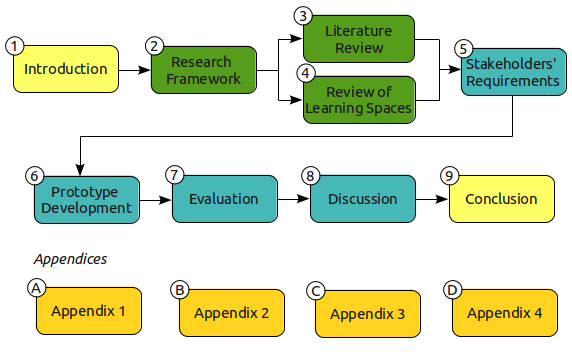
\includegraphics[width=0.9\textwidth]{CH1-F1-Thesis}
\caption{Thesis structure}
\label{fig:ts}
\end{figure}

\begin{description}
\item[Chapter 2.] This chapter presents a methodological approach employed in
this research. Theoretical background of design science research methodology is
given and the way this approach was adopted in this project is described.
\item[Chapter 3.] This chapter focuses on discussing the background of
\LLLsn. Its connection to universities, the current situation in this area and
the problems associated with \LLLs in universities are shown here.
\item[Chapter 4.] This chapter explores the technical worlds of learning
support. System that are currently employed at universities are examined according
to their compliance with \LLLs support.
\item[Chapter 5.] The results of literature review (Chapter 3) and a review of
learning spaces (Chapter 4) are taken to the stakeholders for analysis of their
needs and requirements. Later these findings are used in development of a
conceptual model of an environment that can provide support for \LLLsn.
\item[Chapter 6.] A prototype implementation (based on the requirements
developed in Chapter 5) process and outcomes are presented in this chapter.
\item[Chapter 7.] This chapter describes a complex evaluation design used in the
research to address the questions of quality, functionality and suitability of
the developed features.
\item[Chapter 8.] In this chapter the results and lessons learnt are discussed
with an attempt to analyse issues and question the outcomes. Technical
considerations and practical applications of this research are presented.
\item[Chapter 9.] This chapter brings conclusions and contributions of the
research presented in this thesis. It explores implications for theory and
practice as well as the potential for future research.
\end{description}

This thesis also includes a number of appendices, namely:

\begin{description}
\item[Appendix A] provides ethics documentation for the first stage of the
requirements analysis.
\item[Appendix B] gives an overview of the documents used in the stakeholders
interviews, such as questions used in the interviews and scenarios discussed
with the participants.
\item[Appendix C] consists of the formal requirements specification used for
development of the prototype features. This specification is developed in the
form of user stories.
\item[Appendix D] includes interface screenshots of the prototype features. 
\item[Appendix E] provides ethics documentation for the evaluation stage of this
research project.
\item[Appendix F] overviews the documents used in evaluation Study Two (group
experiment) which includes study protocol, background and exit questionnaire,
participants' responses and the examples of their work.
\item[Appendix G] overviews the documents used in evaluation Study Three (case
studies) which includes study protocol, background questionnaire, and interview
questions.
\end{description}
\chapter{Research Framework\label{cha:method}}
%3100
The main purpose of this chapter is to describe a research approach used in this
study. The first section of the chapter identifies the objectives that need to
be addressed in order to achieve the goal of this study, followed by the research
questions in Section \ref{sec:questions} raised from these objectives.

Design Science Research (DSR) methodology was adopted by this study as the main
research methodology to address the research questions. This methodology
emphasizes the problem-solving and performance-improving paradigms and is
oriented towards creating and evaluating IT artifacts \citep{Hevner2004}. A
five-stage research project framework is outlined in Section \ref{sec:method}
which explains each stage of the project and the methods applied. Methodological
limitations are brought to considerations in Section \ref{sec:limits}. This
chapter concludes with the discussion of related work and projects carried out
in the area of \LLLsn.

\section{Research Objectives}

Understanding how \LLLs in universities can be effectively supported using
technical solutions is an overarching goal of this research. This goal brings up
a number of objectives that need to be addressed:
\begin{description}
  \item[Objective 1.] To determine student and institutional requirements for a
  \LLLs environment within the university context.
  \item[Objective 2.] To identify shortcomings and map these requirements
  against the systems already used in universities to support \LLLsn.
  \item[Objective 3.] To design and implement the features required in an
  environment that supports \LLLs to satisfy the defined requirements.
  \item[Objective 4.] To evaluate how this environment meets the needs of all
  stakeholders in supporting \LLLsn.
\end{description}

\section{Research Questions}
\label{sec:questions}
Based on the objectives, this study addressed the following research questions
supported by sub-questions:

\begin{description}
  \item[RQ1:] \textit{What is the concept of \LLLs and its connection to 
  universities?}
	\begin{itemize}
	  \item What is the role of \LLLs in the university context?
	  \item What is the motivation of universities in supporting \LLLsn?
  	  \item What are the existing university policies for supporting \LLLsn?
      \item What are the components of \LLLs environments in universities?
      \item What are the requirements for successful \LLLs support in
   universities?
	\end{itemize} 
	
   \item[RQ2:] \textit{How are available e-tools used to support \LLLs within
   the university context?}
	\begin{itemize}
		\item What e-tools are currently available to support \LLLsn:
			\begin{itemize}
				\item in general?
				\item in universities?
			\end{itemize}
		\item What are the conceptual strengths and weaknesses of these e-tools in
		university context?
		\item What is the relationship between LMS and e-tools support for \LLLs in
		university context?
	\end{itemize}

	\item[RQ3:] \textit{How can LMS and/or \ep~systems be extended to support
	students in the university context for \LLLsn?}
	\begin{itemize}
		\item What features are available now in these systems?
		\item What are the students and institutional requirements for LMS and
		\ep~to support \LLLsn?
		\item How can these requirements be translated and implemented into new or
		improved features?
	\end{itemize}

	\item[RQ4:] \textit{How does this extended environment meet the needs of 
	stakeholders in university teaching and learning contexts?}
	\begin{itemize}
		\item How can lecturers use new features to provide students with their
		guidance and help them to understand \LLLs skills?
		\item How can students address \LLLs skills using new features?
		\item How can new features help students track their learning progress, manage
		\ep~knowledge and content, demonstrate and share their achievements with
		others?
	\end{itemize}
\end{description}

\section{Research Approach}
\label{sec:method}

Finding the most efficient research approach is an important part of any
research study. A properly selected approach helps to obtain answers to the
research questions while working within the framework that uses methods that
have been verified and tested for validity \citep{Kumar2005}. Multi-paradigmatic
field of ICT offers a number of methodologies (e.g., theory building and
testing, action research, interpretive research, grounded theory, etc.) drawn
from the variety of research philosophies \citep{Vaishnavi2007}. This study
follows design science research methodology that has become popular over the
last five decades as fundamentally a problem-solving approach \citep{Cross1993}.

\subsection{Design Science Research Methodology}

According to \citet{Peffers2008}, design science research (DSR) originates from
engineering and computer science where design is a component of the research
process. \citet[p.~4]{Iivari2009} define DSR as \inlinequote{a research
activity that invents or builds new, innovative artifacts for solving problems
or achieving improvements}. Unlike software development methodology that
does not necessarily need any underlying theory, design science requires a
theoretical foundation for research \citep{Gero1999}. This approach is used in
ICT where there is a need to extend the existing boundaries of the current
systems or to address the important problems by creating new solutions and
artifacts \citep{Hevner2004}. The artifacts can be described as constructs
(vocabulary of a domain), methods (algorithms), models (abstractions),
instantiations (prototype systems), and better theories \citep{Hevner2010}. 

Requirements for DSR project contribution, defined by \citet{March2008}, include
(1) identification of a problem, (2) demonstration that there are no existing
adequate solutions in the area, (3) development of an innovative artifact that
addresses the problem, (4) evaluation of the artifact, (5) communication of the
knowledge added to the area, and (6) understanding of the implications for
theory and practice.

This set of requirements closely resembles the DRS methodology process described
by \citet{Peffers2008} (see Figure \ref{fig:peffers}) and research model phases
found in \citet{Vaishnavi2007} (see Figure \ref{fig:vaishnavi}).

\begin{figure}[h!]
\centering
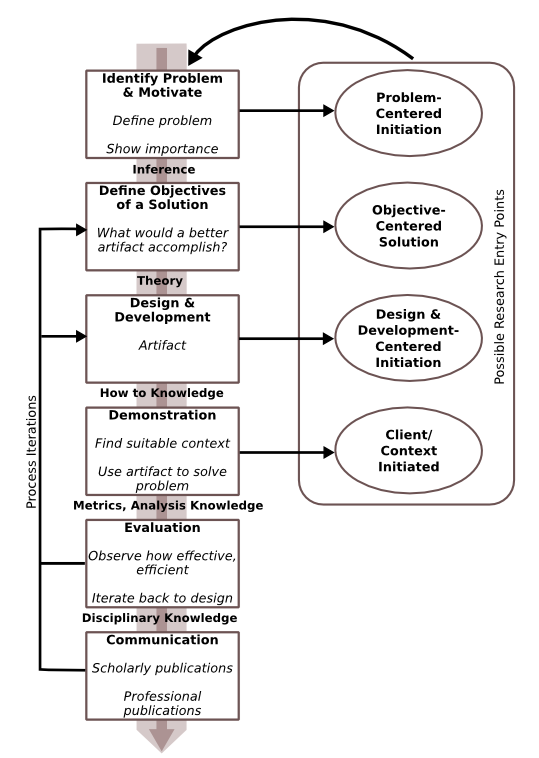
\includegraphics[height=0.76\textheight]{CH2-F1-Peffers}
\caption[Design Science Research Methodology Process Model]{Design Science
Research Methodology Process Model \citep{Peffers2008}}
\label{fig:peffers}
\end{figure}

\FloatBarrier

\begin{figure}[htp]
\centering
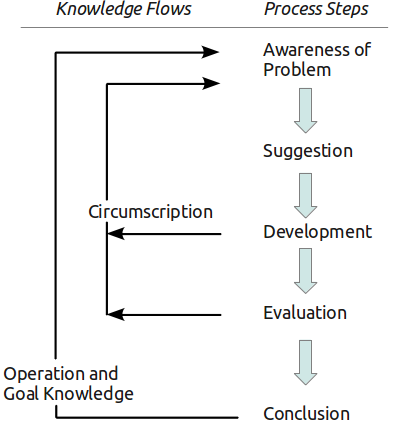
\includegraphics[width=0.5\textwidth]{CH2-F2-Vaishnavi}
\caption[Design Science Reseach Cycle]{Design Science Research Cycle
\citep{Vaishnavi2007}}
\label{fig:vaishnavi}
\end{figure}

All authors essentially agree on common elements. The initial stage of research
is \textit{problem identification} or \textit{awareness}, where a specific
research problem should be stated and the importance of its solution should be
justified. After the problem is identified, the next step is to \textit{suggest
a solution} and define its objectives. This includes understanding the state of
the problem and current available solutions, if any, and explaining how new
solution is going to address the problem in a better way. 

\FloatBarrier

The core phase of research is \textit{design and development}. Conceptually,
this phase consists of deciding the artifact's functional requirements or its
architecture and afterwards creating artifact itself. \citet{Peffers2008} note
that in some cases an artifact is not necessarily a new development. It might
have been already used in another research domain to solve a different problem.

Unlike Vaishnavi's research cycle where evaluation is one step of research
process, Peffer's model distinguishes between \textit{demonstration} and
\textit{evaluation} of the artifact. Demonstration is used to show that the
implemented idea works, while evaluation is a more formal form of measurement of
how well the artifact supports a solution to the problem \citep{Peffers2008}.
Artifact can be evaluated from various perspectives such as performance,
usability, reliability, accuracy, quality, functionality, etc.

The last stage of research is \textit{conclusion} or \textit{communication}. It
might involve but is not limited to: discussing the problem, its importance, the
novel artifact, and its effectiveness with relevant research audiences; creating
scholarly publications; presenting research findings at the conferences; and
writing a project report \citep{Archer1984}. However, if no satisfying results
have been reached at this stage of the research cycle, it might as well serve as
a subject for further research.

Described in Table \ref{tab:guidelines} are seven guidelines identified by
Hevner \citeyearpar{Hevner2004} that should be followed by the beginning
researches for effective DSR.

\begin{table}[htb]
  \caption[Design Science Research Guidelines]{Design Science Research
  Guidelines \citep{Hevner2004}}
  \begin{center}
    \begin{tabular}{| l | p{6.5cm} |}
    \hline
     \multicolumn{1}{|c|}{\textbf{Guidelines}} &
     \multicolumn{1}{c|}{\textbf{Description}} \\
     \hline
     Guideline 1: Design as an Artifact & Research must produce a viable
    artifact such as a construct, a model, a method or an instantiation \\ \hline
     Guideline 2: Problem Relevance & Research must develop technology-based
     solutions to important and relevant problems \\ \hline 
     Guideline 3: Design Evaluation & Proper valuation methods must be used to
     demonstrate artifact's quality and efficacy \\ \hline 
     Guideline 4: Research Contributions & Research must provide clear
     contributions to the research areas \\ \hline 
     Guideline 5: Research Rigor & Rigorous methods must be applied to
     construction and evaluation of the artifacts \\ \hline 
     Guideline 6: Design as a Search Process & Research must incorporate a
     search process to find and effective solution to the problem \\ \hline
     Guideline 7: Communication of Research & Research must be effectively
     communicated to relevant audiences \\ \hline
    \end{tabular}
  \end{center}
  \label{tab:guidelines}
\end{table}

In contrast to Hevner, \citet{Venable2010} argues that there is no common
understanding of what kind of guidelines and standards should be used for
effective DSR. However, based on analysis in the same work, the majority of
respondents who are researchers and DSR practitioners agree on a few points: DSR
should address important problems, have an artifact that would help to solve the
problem, and have some kind of evaluation of this artifact.

\subsection{Design Science Research Applied to This Project}

The research framework in the current research is adapted from a DSR cycle
established by \citet{Vaishnavi2007}. They identify five phases in the research
model: (a) identification of a problem, (b) suggestions and objectives of a
solution, (c) design and development, (d) demonstration and evaluation, and (e)
conclusion and communication.

\begin{figure}[htb]
\centering
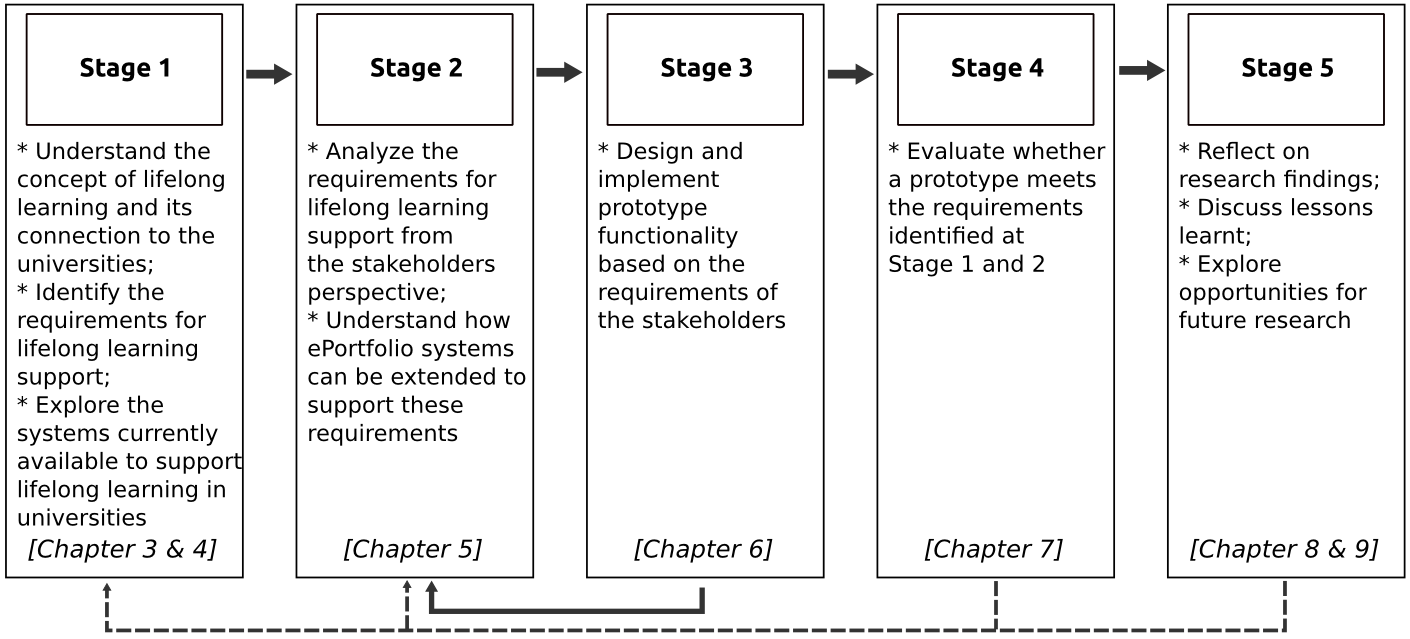
\includegraphics[width=1\textwidth]{CH2-F4-Path}
\caption{The research path}
\label{fig:path}
\end{figure}

Figure \ref{fig:path} shows a research path of this project from the first
to the last stage. It can be seen that at the later stages of the project it was
necessary to look back and reflect on findings in order to understand whether
the research objectives were met and what lessons were learnt. Other iterations
in this project were between stages three and two where the prototype had to be
taken back to the stakeholders for feedback. Although, according to Figures
\ref{fig:peffers} and \ref{fig:vaishnavi} the end of the evaluation can be
considered another potential stage to iterate back, \citet{Peffers2008} says
that the nature of the research project usually shows whether iterating back is
feasible or not. In this case, due to the time and resources constraints,
further improvements were left to the subsequent research projects.

\subsubsection{Stage 1. Problem Identification and Motivation}

Any research project can be started either from the gap in the literature or
when a problem that is worth solving exists \citep{Bourner2002}. Previous
experience and observations of the existing problems in the field of study
formed the background for this research. To define the main research topic,
preliminary investigations were made as part of the field of study review. The
problem identified in the current research is the difficulty in supporting
students' \LLLs in universities. Defining the research topic led to the research
questions and objectives development which, in turn, formed the direction and
focus of this project.

\subsubsection{Stage 2. Objectives of a Solution}

To answer the research question on the concept of \LLLs and what kind of
environment can support it, it is important to develop understanding of
current theories and practices of \LLLs support. A comprehensive literature
review and a review of the learning spaces was undertaken to address these
questions.

However, this research did not rely on a literature review alone. A set of
interviews with the stakeholders were organized to support literature findings
and identify the gaps that exist in current \ep~systems. Interviewees were
asked to look at the \ep~system from the \LLLs perspective and offer their
solutions for supporting guiding principles and recommendations for successful
\LLLs discovered in the literature.

Interviews were audio recorded, transcribed and analyzed. The results were
compiled into a set of formal software requirements specification to be
implemented in a system prototype for the future evaluations.

\subsubsection{Stage 3. Design and Development}

In the development phase, the results of the literature review, interviews and
requirements analysis were used to create a conceptual model of an \ep-supported
environment that can facilitate students in \LLLs and be compatible with
university needs.

A functionality, based on this model, was implemented in a prototype \ep~system.
As the requirements specification was too large for a project of limited size
and within a relatively short timeline, only high priority requirements were
implemented. The requirements were prioritized according to the feedback given
by the interviews participants at the initial stages of the project. Due to
this, a number of requirements related to a better integration of the
\ep~systems with LMS and usability improvements were omitted. Although these
requirements were not implemented, they were still included into the conceptual
model.

Prototyping followed established software engineering practices that interleaved
coding and revision, forming iterative development cycles, as shown in Figure
\ref{fig:prototype}.

\begin{figure}[htb]
\centering
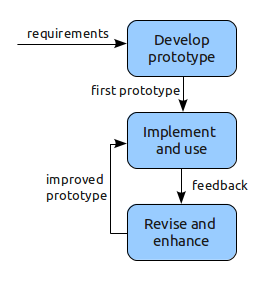
\includegraphics[height=0.3\textheight]{CH2-F3-Prototype}
\caption[Prototyping]{Prototyping based on \citet*[p.~411]{Sommerville2007}}
\label{fig:prototype}
\end{figure}

After each iteration was completed, the prototype was taken back to the
stakeholders for feedback. This was necessary to understand what changes were
required and to design further improvements. These iterations are shown on
Figure \ref{fig:path}.

Mahara \ep~system\footnote{\url{http://mahara.org}} was used as an initial base
system for the prototype. There is a number of reasons why this system was
selected. Mahara is a trusted and widely-used in universities (and at Massey
University in particular) solution with a large community support. This system
is open source which makes it easy to access and allows modifications like
adding new features and changing the existing ones. Mahara is a \textit{typical}
representative of its category and provides all commonly available features. At
the same time it is a leading edge system developed by using latest web
technologies and programming practice.

\subsubsection{Stage 4. Demonstration and Evaluation}

It is important for evaluation to be treated not as an isolated process, but as
a part of design process \citep{Cleven2009}. Although, the prototype was
reviewed by the stakeholders after every development cycle, a formal evaluation
of the overall concept was still required.

It is not likely that a single evaluation technique can establish effectiveness
and value of the prototype in a complex area of \LLLsn. In such cases it is
recommended \citep{Quinlan2008} that the evaluation design should incorporate a
variety of methods, that taken together can provide reasonable evaluation
outcomes.

Due to time and resources constraints, and an extended \ep~system being a
functional prototype, it was not feasible to conduct evaluations in the real
world settings. However, it was possible to develop a number of studies that
looked into the specific aspects of \LLLs support and evaluated how well
developed features satisfy the requirements identified earlier by the
stakeholders.
 
As a result, features implemented in the prototype were evaluated from three
different perspectives: 

\begin{itemize}
  \item Demonstrations of the prototype and its extended functionality were used
  for exploratory evaluation with the lecturers. The aim was to explore how the
  lecturers can integrate new features into their teaching to provide students
  with guidance and help them to understand \LLLs skills.
  
  \item An experiment with various representatives of undergraduate students
  was undertaken to understand how added functionality can help them to address
  institutional graduate attributes and \LLLs skills. Thirty five students with
  different levels of knowledge of \LLLs skills and experience of using
  \ep~systems were involved in the experiment.

  \item Case studies were used to evaluate the prototype from the mature
  students' perspective. This approach was selected due to its internal and
  external validity, control and in-depth examination of each case \citep{Yin2009}.
  Participants with different study backgrounds had access to the prototype for
  an extended trial period of time and were able to get a better look at the new
  features. At the end of the trial period, each participant was interviewed and
  gave their feedback on the features they had used.
\end{itemize}

\subsubsection{Stage 5. Conclusion and Communication}

Where it was possible the results of the various stages of this research project
were documented and submitted for publications and conference presentations. A
full list of publications can be found in \hyperref[sec:pub]{Publications and
Presentations} section of this thesis.

\section{Methodological Limitations}
\label{sec:limits}

Any study and its findings should be weighed against methodological
limitations. Acknowledging limitations is important for scientific progress as
they might help to understand how research can be improved in the future
\citep{Ioannidis2007}. Although, literature does not explicitly describe
limitations of DSR methodology, they can still be derived from the limitations
of the methods used at each stage of the study. Therefore, the limitations
considered in this research included:

\begin{description}
\item[Sample size:] Sample size for Stage 2 was relatively small due to the
participants profile requirements. In addition, the snowballing sampling
technique was used to find suitable student participants which might have
influences the outcomes of this stage.
\item[Prototyping:] The evaluated system was a prototype based on the open
source \ep~system Mahara which might have led to biased feedback as some
participants were familiar with the system and already had their opinions about
it.
\item[Evaluation:] Due to the nature and scale of this research project, its
time and resources constraints, evaluation was not conducted in real world
settings. Alternatively, a set of case studies, an experiment and exploratory
evaluations have been undertaken.
\end{description}

A more detailed discussion of the limitations can be found further in the
relevant chapters of this thesis.

\section{Related Work}
\label{sec:related}
As \LLLs concepts gained general acceptance, there were a number of studies
aimed to explore \LLLs support in various contexts. To date, research similar to
this project has not been identified, although projects found were a valuable
source of information and examples of previous research experience.

\begin{itemize}
  \item Lifelong Learning in London for
  All\footnote{\url{http://www.lkl.ac.uk/research/l4all.html}} (L4All): This
  project is focused on developing of \LLLs system to support independent
  learners (particularly those 16+ learners who traditionally have not
  participated in higher education) by recording their learning pathways. This
  project aimed to provide lifelong learners in the London region with access to
  information and resources that facilitates their progression from secondary
  education to further education or from secondary education directly to higher
  education \citep{Freitas2006};

  \item The Regional Interoperability Project on Progression for Lifelong
  Learning\footnote{\url{http://www.nottingham.ac.uk/rippll}} (RIPPLL): This
  project was going to establish a model of cross-sector collaboration in
  personal development planning technology in the UK. The aim was to make all
  the major existing electronic systems interoperable for study-based progress
  files that are used in further and higher education to provide an easier
  transition process from school to further education \citep{Hartnell-Young2006};

  \item ELGG-Moodle: In autumn 2006 Klagenfurt University, Austria was piloting
  the project that aimed to integrate Moodle LMS and ELGG platform. This
  integration was used for professional development for all academic staff.
  Project outcomes provided integration between systems such as single login and
  file transfer \citep{Attwell2007}.

  \item Accessible \LLLc for Higher
  Education\footnote{\url{http://www.eu4all-project.eu}} (EU4ALL): A project
  started in 2006 that aimed to develop components and services for universities
  to make learning more accessible for both the students with functional
  diversity and the elderly. This project looked into providing better access
  to the electronic content and educational resources in higher education using
  a framework or a set of free tools that support mobile learning, audio
  recording transcription, DAISY digital books and other adaptations of contents
  based on the student's needs and preferences.

  \item An \ep~based Pedagogy for Small to Medium-sized
  Enterprises\footnote{\url{http://www.wlv.ac.uk/ePPSME}} (ePPSME): Finished
  in 2011, this project provided higher education sector with reusable models
  for an \ep-based pedagogy for work-based learners. This pedagogy addresses
  the needs of learners with shortage of time, previous informal learning
  experience, need for flexible delivery and quality of learning, and
  opportunities to record achievements \citep{Felce2011}.
\end{itemize}

Unlike this research, the majority of above described project were focusing
either on collaboration between sectors (school -- university or university --
workplace) or were aimed at developing of theoretical rather than practical
solutions. The ELGG-Moodle integration project was the most relevant in
the technical context of this research, however it focused on not students,
but staff development. 

As well, these project were analysed with the intention of adopting a suitable
evaluation design. However, an approach feasible for the research of this size
and timeframe has not been found among the previous projects.

\section{Summary}

To address the objectives and research questions stated at the beginning of the
chapter, this research project follows DSR methodology. DSR is a problem solving
approach that focuses on development and evaluation of innovative IT artifacts.
This chapter outlined a five-stage research framework used in this work with
each stage explained.

The next chapter will explore the literature review undertaken to understand the
concept of \LLLs and the requirements for its efficient support. It will provide
a background for the further theory development of this research.
 
\chapter{Literature Review - Lifelong Learning \label{cha:litrev}}

In order to answer the first research question, it is important to establish a
basic understanding of the main concepts used in this work. Although,
underlying concepts can be found primarily in the domain of education, they make
a good starting point for a discussion. 

This chapter introduces the key concept of \LLLs that will be in focus
throughout the thesis. First, the origins of the term of ``\LLLsn'' and related
concepts are discussed in Section \ref{sec:concepts}. The crucial differences
between these concepts and how they transformed over time, driven by changing society and
economics, are explored. Second, through the increasing focus on \LLLs skills in
the world of work and in higher education, Section \ref{sec:uni} shows the need
for \LLLs support in universities. Universities are in center of this
dicussion as they provide the necessary organizational framework, theoretical
principles and practical experience for \LLLs \citep{Knapper2000}, which can be
seen in the role and influence of the universities in the educational systems of
most countries as the ``keepers of the intellectual traditions of a nation"
\citep[p.~96]{Longworth2003}. Third, in Section \ref{sec:needs} the general
needs for successful \LLLs are outlined. No explicit requirements have been
found in the literature. However, commonly accepted recommendations and
guidelines were discovered in various sources that will be used as a background
for further exploration in Chapter \ref{cha:model}.

\section{Literature Review Process}
The literature review on \LLLs (Chapter \ref{cha:litrev}) and a review of
institutional and open learning spaces (Chapter \ref{cha:systudy}) that provide
and support background for this thesis were conducted by systematically reading
and reviewing books, journals and conference proceedings in the area of
research. The main methods to identify relevant literature were recommendations
of domain experts and a library search. Relevant articles were identified by
reading titles and abstracts of selected journal articles and papers in
conference proceedings. Where possible the latest ten years of issues of the
following journals were looked through: ``British Journal of Educational
Technology'', ``International Journal of Lifelong Education'', ``European
Journal of Education'', ``\LLLc in Europe'', ``International Journal of Emerging
Technologies in Learning'', ``New Zealand Journal of Adult Learning'', ``Journal
of Computer Assisted Learning'', ``European Journal of Engineering Education'',
and ``International Journal of ePortfolio''. In addition, a keyword search was
carried out on the Internet and academic resources (such as Education Research
Complete\footnote{\url{http://www.ebscohost.com/academic/education-research-complete}},
Academic Search
Premier\footnote{\url{http://www.ebscohost.com/academic/academic-search-premier}},
Directory of Open Access Journals\footnote{\url{http://www.doaj.org}},
Google\footnote{\url{http://google.com}}, Google
Scholar\footnote{\url{http://scholar.google.com}}) to cover conference
publications not available in the library. The following keywords and
combinations of keywords were used in the search: ``\LLLsn'', ``life-long
learning'', ``e-learning'', ``ePortfolio'', ``e-portfolio'', ``electronic
portfolio'', ``Web 2.0'', ``learning environment'', and ``learning
technology''.

This review helped to discover previous work in the area (described in Section
\ref{sec:related}), explore methods that could be applied to this research,
increase the depth and breadth of knowledge of the field, and identify domain
experts and other people working in the same field who could be valuable to
contact. Besides finding relevant information in the literature, it was also
notable to identify the gaps that currently exist (more detailed discussion can
be found in Chapter \ref{cha:systudy}). It will be shown further that these gaps
are based on facts that although a lot of work has been done on developing \LLLs
theories as well as developing technologies for education and learning, there is
little substantial work done on combining these two areas.

As a continuous process, the literature review for this research was updated by
actively acquiring and reading the relevant articles emerging in the literature.

\section{The General Concept of \LLLc}
\label{sec:concepts}
\subsection{Terms and Definitions}

The European Commission \citeyearpar{EuropeanCommission2000} defined \LLLs as:

\longquote{All learning activity undertaken throughout life, with the aim of
improving knowledge, skills and competencies within a personal, civic, social
and/or employment-related perspective.} 

However, it is not as simple as it looks: the concept of \LLLs consists of a
variety of meanings, models and ideas. Such terms as '\LLLsn', 'lifelong
education', 'adult education', 'recurrent education', 'continuing education',
and 'further education' create a set of to some extent related, yet different
concepts \citep{Hager2011}.

'Continuing education' (also referred to as 'adult education') was introduced in
the late 1970s and early 1980s. There was no common definition of this term,
but in some sources  \citep{Jarvis2004} it was described as all learning
activities which could be undertaken after compulsory schooling is finished.
Figure \ref{fig:learning} compares the main concepts in education according to
the time spent by individuals learning/studying across their lifespan. As can be
seen, continuing education was usually part-time and accured less frequesntly
than other forms of education.

\begin{figure}[htb]
\centering
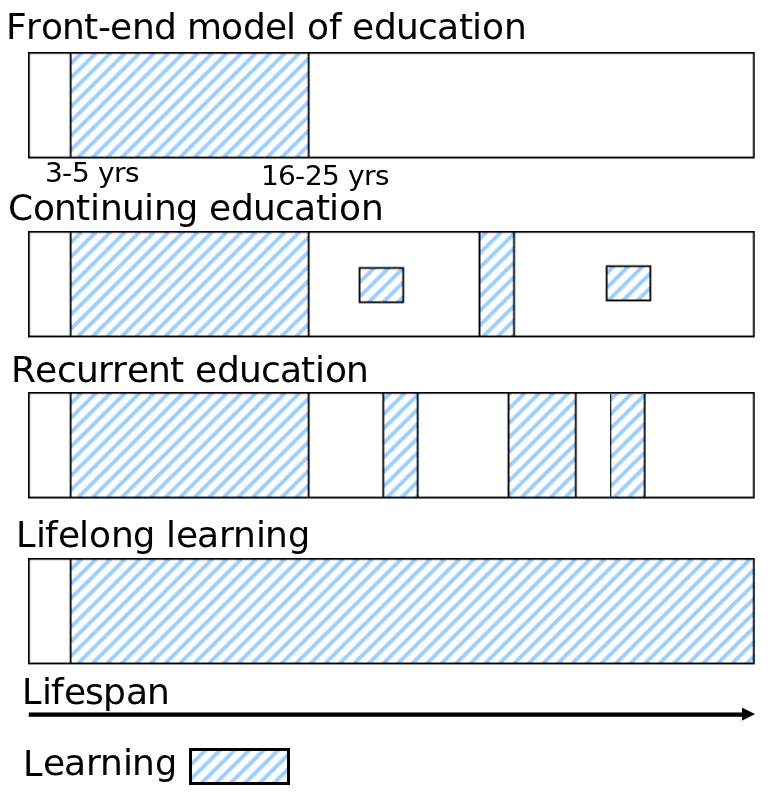
\includegraphics[width=0.55\textwidth]{CH3-F1-Learning}
\caption[Changing concepts of learning]{Changing concepts of learning 
\citep{Jarvis2004}}
\label{fig:learning}
\end{figure}

The term 'recurrent education' was widely used by OECD until the 1980s
\citep{Jarvis2004}. Unlike intermittent continuing education, its idea was
in allowing adults to spent full time studying in formal education sector doing
on-the-job trainings or post-compulsory education of any kind. Arguably, this
main feature of the right for full time study made the concept of recurrent
education disappear from the governments' eduactional agendas: it was too
expensive and difficult to support this policy.

Rejecting the concepts of recurrent and continuing education played an important
role in development of the new educational models. While they had different
undelying  philisophy, they both recognized the fact that aquisition of
knowledge should be a lifelong process, from ``cradle to grave''
\citep{Hargreaves2004}.

The origin of the term '\LLLsn' goes back to the early 20th century and is
contributed to by John Dewey \citeyearpar{Dewey2004}. From his perspective,
\LLLs had to be centered on the individual's ability to take an active role in
democratic society. He saw education as a learning process which was influenced
by the growth of the individual and society, both interlinked. Dewey's key to
\LLLs was in developing active learning, enabling the individual to reflect and
change throughout life, emphasizing that non-formal education was as important
as formal education.

The concept of 'lifelong education' was discovered in 1972 after Edgar Faure's
Report ``Learning to Be'' for UNESCO. The concept described in the report was
announced to be the leading one for the reform in education. Faure's Report used
four principles for the lifelong education architecture \citep{Faure1972}:
vertical integration (education should occur throughout one's life), horizontal
integration (acceptance of non-formal and formal education), the democratization
of education (more widespread involvement of learners) and learning society
(restructuring of educational system). However, according to Hager's
\citeyearpar{Hager2011} analysis, UNESCO's concept of 'lifelong education' put
the emphasis on formal education as the only sufficient and relevant form of
learning to provide actual 'education'.

\subsection{Paradigm Shift and \LLLc Today}

Almost 40 years after the idea of this lifelong education was introduced, many
governments rediscover not lifelong education, but \LLLs \citep{Boshier2000}.
This shift was not only semantic, but also substantive, which showed that \LLLs
and lifelong education are not the same: lifelong education aimed to develop
more humane individuals and communities, while \LLLsn's goal was in retaining
and gaining new skills that would help individuals adapt to rapid changes in
their workplace \citep{Medel-Anonuevo2001}. Lifelong learning is based on the
notion of the individual learner as a consumer. And as a result if consumers
decide not to take advantage of all the opportunities they have -- then it is
their fault. Therefore, being constructed as individual activity, learning
depends entirely on personal motivation. Unlike learning, education is a
provided service \citep{Boshier2000} that requires someone to be responsible for
providing resources, developing policies, etc. The emphasis on 'learning' rather
than 'education' is significant \citep{Tuijnman2002}, as it moves focus from the
institutions onto the individual. Although, it does not mean that institutions
and govermnets play no role whatsoever. Their role is rather transformed into
investment in individuals and creation conditions for them to take charge of
their learning \citep{Chen2009}.

Over the last decade, lifelong learning support has become a part of official
government policy in a number of countries around the world. As an example,
European Commission has established a budget of nearly 7 billion Euro for the
period of 2007-2013 for 'Lifelong learning programme' which aims to support
education and training at school, college, university, in the workplace and in
the community across Europe \citep{TheEducation2009}. In New Zealand a number of
governmental documents \citep{NewZealandMinistryofEducation2008} now mention
the ``success of all New Zealanders through lifelong learning". As a result, the
national tertiary education system of the country has been transformed to
support lifelong learning ideals \citep{Benseman2006}.

\begin{figure}[htb]
\centering
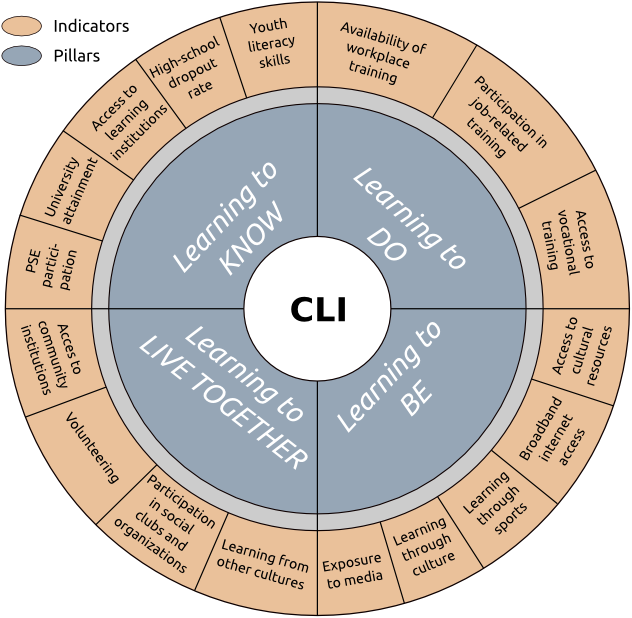
\includegraphics[width=0.8\textwidth]{CH3-F2-CLI}
\caption[The 2010 Composite Learning Index of Canada]{The 2010 Composite
Learning Index of Canada}
\label{fig:cli2010}
\end{figure}

In 2006 Canadian Council on Learning developed the 17 indicators and 26
specific measures (Figure \ref{fig:cli2010}) called Composite Learning Index
(CLI) that is used to calculate annual progress in \LLLs in the country
\citep{CanadianCouncilonLearning2011}. Using CLI, Canadian government expects to
draw attention to the benefits of \LLLs and demostrate learning opportunities
that occur outside of classroom settings. In August 2010 European Union adopted
this Index as European \LLLc Indicators (ELLI). Similar to CLI, ELLI were using
UNESCO approach of four pillars of learning: Learning to Know, Learning to Do,
Learning to Be, and Learning to Live Together \citep{ELLIDevelopmentTeam2010}.

\subsection{Components and Attributes of Lifelong Learning}
In terms of purposeful learning activities \LLLs consists of the following
components \citep{Longworth2003, Tuijnman2002}:

\begin{itemize}
  \item Formal learning -- institutionally graded, and hierarchically structured
system, often leads to qualification;
  \item Non-formal learning -- organized systematic educational activity
  external to formal education;
  \item Informal learning -- planned or not planned, but conscious learning from
the experience;
  \item Incidental learning -- not intentional, an accompaniment to everyday
  life, learning during the action.
\end{itemize} 

\begin{figure}[htb]
\centering
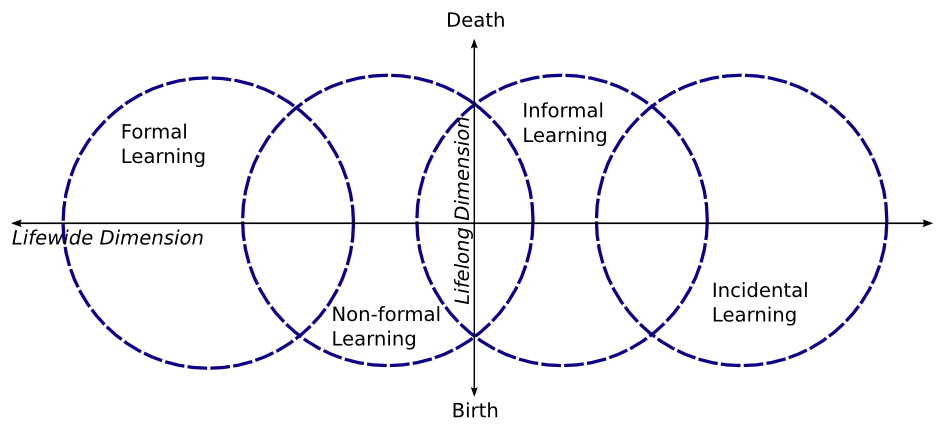
\includegraphics[width=0.8\textwidth]{CH3-F3-LLLFramework}
\caption[Framework for \LLLc]{Framework for \LLLc (based on
\citet[p.~11]{Divjak2004})}
\label{fig:lllfmwrk}
\end{figure}

Some researchers \citep{Longworth2003} recognize only two categories of lifelong
learning, formal and non-formal, leaving informal and incidental parts of it as
the elements of non-formal learning. Boshier \citeyearpar{Boshier2000} states
that the current reality is such that the formal and non-formal categories of
\LLLs are like ``two parallel railway lines. Both cross the landscape but never
touch'' (p. 11), explaining this way that formal setting have practically
nothing to do with non-formal.

From another perspective, \LLLs encompasses the elements of self-direction,
long-term and life-wide learning \citep{Schuetze2006}. Rubenson
\citeyearpar{Rubenson2002} called these 'three fundamental attributes of \LLLs':

\begin{itemize}
  \item Lifelong -- means everything from cradle to grave;
  \item Life-wide -- takes place outside the formal education system;
  \item Self-directed -- is guided by the learners themselves and does not
  limit itself to education.
\end{itemize} 

Weert and Kendall \citeyearpar{Kendall2004} gathered other essential
characteristics of \LLLsn:

\begin{itemize}
  \item Most of \LLLs occurs outside of classroom as is not triggered by
  textbooks;
  \item The driving force in \LLLs is self-motivation and active participation
  of learners;
  \item Lifelong learning involves interactions, groups, community learning and
  other social activities;
  \item Solving atrificial tasks does not matter in \LLLsn. Achievements in
  real-life situations measured by common standards are important;
  \item Lifelong learning is learner centred and aims for personal
  achievements;
  \item Lifelong learners should maintain their achievements portfolio.
\end{itemize} 

These characteristics describe \LLLs as demand-driven, flexible, social and
personal at the same time. Hereinafter, any further reference to \LLLs will be
made in terms of the concepts outlined in this section.

\section[\LLLc in Universities]{\LLLc in Universities\footnote{This section was
adopted from the section originally published as part of Chapter 8 ``The Role of
Institutions in Creating Student-Focused Virtual Learning Spaces with ePortfolio
Systems'' of the book ``Physical and Virtual Learning Spaces in Higher
Education: Concepts for the Modern Learning Environment". Full reference can be
found in Publications section.} }

\label{sec:uni}

As \LLLs consists of the concepts of 'life-long', 'life-wide' and 'self-
directed' learning, it has following significant implications. As already
mentioned above, 'life-long' means the full life span of an individual. From the
institutional view it starts when students are enrolled in the university and
finishes when they graduate. 'Life-wide' component of learning implies that
learning can and should occur not only as formal university study, as personal
and professional development takes place in many contexts. Attwell
\citeyearpar{Attwell2007} considers the fact that everyday non-formal types of
learning are not connected to institutional formal education to be the major
issue of modern learning, which can make students see their study at university
as ``something irrelevant to their identities'' (p. 4). For successful \LLLs,
progress of the achievements should be recorded and maintained over a long
period and across various sources, formal as well as non-formal \citep{Kay2008}.
A \LLLs environment needs to acknowledge this and allow learners to record and
reflect on experiences from all these contexts.

Over recent years the skills that provide \LLLs ability were identified, they
include: solving problems, critical thinking, utilizing technology, and
information literacy; working with others in teams, communication skills,
leadership and social interaction skills; self-management; collecting, analyzing
and organizing information; planning and organizing activities; cultural
awareness and understanding
\citep{Brooks2008,Heinrich2007,Otala1997,Pitman2009}. The importance of these
skills in addition to academic and subject knowledge has been increasingly
emphasized in the workplace and public policy
\citep{Morgan-Klein2007,Sutherland2006}. Individuals today need to continue to
update and upgrade their skills and knowledge even after completing formal
education in order to survive in the changing world. Otala
\citeyearpar{Otala1997} states that required flexibility and adaptability to
these rapid changes are gained through ``better developed learning skills and
the right attitudes that help individuals quickly and easily learn new things''
(p. 456). Therefore, current students need to ``possess something more than
skills which grow obsolete as technology advances'' \cite[p.~195]{Field2003}. 

Higher education institutions have responded to the need for \LLLs skills by
defining their own strategies to promote \LLLsn. Many institutions in Europe,
the United States, Australia and New Zealand now explicitly express the \LLLs
characteristics they strive for in their graduates \citep{Scanlon2006}.
Australian universities, such as Curtin University, have made policy
declarations committing to graduate attributes across their programmes
\citep{CurtinUniversity2006}. The College of Sciences of Massey University has
formulated a draft \LLLs policy \citep{MasseyUniversity2008} that expresses
values, support and expectations in regards to \LLLsn. Graduate profiles, naming
\LLLs skills such as critical thinking, effective communication, teamwork and
leadership have been established for many degree programme
\citep{Davies2003,McAlister2003}. The accreditation criteria for engineering
degrees now refer to and demand soft skills \citep{Aller2005,Muffo2001}. The
need for a holistic education and the development of students beyond technical
competency is requested \citep{Brakke2002,Davies2003,Dowling2006,Fallows2003,Grabowski2004,Hernon2006}.

In order to enact policy academics need to incorporate development opportunities
for these skills into their teaching and learning designs. While individual
academics succeed in doing so by using techniques such as group work, reflective
journals and authentic assessment \citep{Clarke2003,Lombardi2008}, universities
are far from achieving the required levels of \LLLs skills in their graduates
for the following reasons.

While graduate profiles express graduate attributes and \LLLs skills, the
individual courses making up the degrees have not been adjusted accordingly. One
consequence of this is that students are not presented with a coherent picture
across their courses and that it is too easy to disregard the messages given in
single courses. Some academics may lack awareness, skills and support to fully
incorporate the development of \LLLs skills into their teaching. Academics who
do not consciously practice their own \LLLs skills development will find it
difficult to lead and to inspire their students. Yet, students need guidance in
developing \LLLs skills \citep{Leone2019}, both to recognise their importance
and to acquire the knowledge 'how to' study \citep{Medel-Anonuevo2001}. The
currently dominant academic systems are in conflict with the characteristics of
\LLLs skills. Instead of supporting the needs of learning to be self-directed,
life-wide and lifelong, these systems are assessment-driven and focus on course
content and duration.

\section{Requirements for Successful \LLLc}
\label{sec:needs}
Based on considerations outlined earlier in this chapter, this section brings
together the requirements for provision of successful \LLLs support for
students. Although, no explicit set of requirements has been found, the
literature identifies a number of guidelines and recommendations that have to be
satisfied in order to achieve successful \LLLs support in universities. Some of
them have already been mentioned throughout this chapter.
 
\begin{itemize}
  \item Universities should provide support for all aspects of \LLLs (formal,
  informal, non-formal, incidental); 
  \item Students need guidance on various levels \citep{Leone2019};
  \item Lecturer should be an active facilitator and promote involving learning
experiences \citep{Leone2019}; 
  \item Learning materials should be organized in the way that would help
students learn how they learn \citep{Medel-Anonuevo2001};
  \item Communication and collaboration are essential parts of learning process
  \citep{Schaffert2008};
  \item Learning progress should be recorded from various sources and maintained
  over a long period of time \citep{Kay2008};
  \item Students need to be aware of their personal achievements
\citep{Schuetze2006};
  \item Students should develop understanding and confidence in their knowledge
  and be able to address higher-order skills (graduate attributes in university
  context) \citep{Hart1999};
  \item Students should be able to evaluate and reflect on their own performance
and learning progress \citep{Mourtos2003}.
\end{itemize} 

These theoretical recommendations will be used to guide further exploration of
 how \LLLs can be supported using thechical solutions available in universities.

\section{Summary} 

Following from the discussions in this chapter, it is important to emphasize
the next key points: \LLLs plays an important role in current global economics
and society; \LLLs skills have become a fundamental part of personal
development; governments and educational institutions, universities in
particular, are attempting to promote and support \LLLsn; at this stage, \LLLs
support provided in universities is not sufficient to satisfy the needs of
students as lifelong learners.

In order to support this argument, the next chapter will review the world of
learning spaces that are currently used in universities and outside of
educational sector to support various learning activities. The connection and
gap that exists between these systems from the \LLLs prespective will be
thoroughly explored.

\chapter{Designing Conceptual Model\label{cha:model}}

\section{Summary} 
\chapter{Prototype - Development and Implementation\label{cha:prototype}}

\section{Summary} 
\chapter{Evaluation\label{cha:evaluation}}

\section{Summary}  
\chapter{Discussion\label{cha:discussion}} 
\chapter{Conclusions\label{cha:conclusion}} 

% ========================Appendices================================
\appendix
\chapter{A Typical Appendix...}

...consists of all the junk that you couldn't fit into the main part of the thesis, like more tables of data.


% ========================Bibliography==============================

\addcontentsline{toc}{chapter}{Bibliography}
\bibliography{references}             
\bibliographystyle{bevbib4}%{plainnat}  

\end{document}
